\documentclass[11pt]{article}
\usepackage{fullpage}
\usepackage{graphics,epsfig,color}
\usepackage{wrapfig}
\usepackage{amsmath}
\usepackage{forest}
\usepackage{times}
\usepackage{setspace}
\usepackage{amsmath,amsthm,amssymb}
\usepackage{subfigure}
\usepackage{url}
\newtheorem{problem}{Problem}
\newtheorem{answer}{Answer}
\usepackage{listings}
\usepackage{color}
\usepackage{adjustbox}
\usepackage{tikz}
\definecolor{dkgreen}{rgb}{0,0.6,0}
\definecolor{gray}{rgb}{0.5,0.5,0.5}
\definecolor{mauve}{rgb}{0.58,0,0.82}
\usepackage{graphicx}
\graphicspath{ {images/} }

\lstset{frame=tb,
	language=Java,
	aboveskip=3mm,
	belowskip=3mm,
	showstringspaces=false,
	columns=flexible,
	basicstyle={\small\ttfamily},
	numbers=none,
	numberstyle=\tiny\color{gray},
	keywordstyle=\color{blue},
	commentstyle=\color{dkgreen},
	breaklines=true,
	breakatwhitespace=true,
	tabsize=3
}

\begin{document}
\begin{center}
	{\LARGE CSCD320 Homework7}
	
	\bigskip
	
	{\Large Ethan Tuning}
\end{center}

\bigskip

\begin{problem}
 \label{prob:1}
 Print the BFS and DFS that starts from the vertex d of the following graph. If a vertex has multiple next-hops, then search the next-hops in the order of their vertical coordinates from the lower ones to the higher ones.
\begin{center}
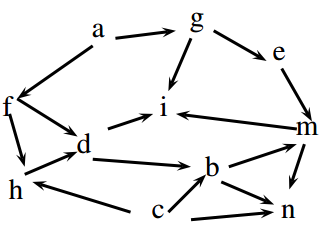
\includegraphics[width=4cm, height=3cm]{graph1}
\end{center}
\end{problem}

\begin{answer}
\label{ans:1}
BFS: d, h, b, f, i, c, n, m, a, g, e. DFS: d, b, i, n, m.
\end{answer}

\bigskip

\begin{problem}
 \label{prob:2}
 Given the adjacency list representation of an unweighted graph G = (V,E), give your pseudocode that constructs the matrix representation of G. Describe the time complexity of your algorithm in the big-oh notation and make your bound as tight as possible.
\end{problem}

\begin{answer}
 \label{ans:2}
 Here is the pseudocode:
\begin{center}
\begin{lstlisting}
 for i = 1 to n
	 for j = 1 to n
		 if j is in i's adjacency list
			 write 1;
		 else
			 write 0;
\end{lstlisting}
\end{center}
 Time complexity will be $O(\log{n})$.
\end{answer}

\bigskip

\begin{problem}
 \label{prob:3}
 The DFS algorithm that we discussed in class uses the adjacency list representation
 of a graph $G = (V,E)$ and its time cost is $O(|V | + |E|)$. Suppose you are only given the matrix representation of G, describe your pseudocode for DFS of G using the matrix representation. Give the time complexity of your algorithm in the big-oh notation and make your bound as tight as possible. Did you learn why we used the adjacency list representation for DFS in class?
\end{problem}

\begin{answer}
 \label{ans:3}
 Here is the pseudocode:
\begin{lstlisting}
	for i = 1 to n
		if visited[i] = 0
			dfs(i); //call to the dfs list version
\end{lstlisting}
Time complexity will be $O(|V|^2)$. This is terrible and we want to use the adjacency list version because it is way faster.
\end{answer}

\bigskip

\begin{problem}
 \label{prob:4}
 In class, we have discussed how to use DFS for topological sorting of a DAG. Someone tries to come up with something new by trying to use BFS for topological sorting of a DAG. Below is his/her code. Does his/her code work ? If yes, explain why? If no, give a counter example.
 
\begin{lstlisting}
	time = 0; //global clock
	//G: the graph. s: the vertex to start with
	
	graph_BFS(G,s) {
		time = time + 1; //New operation
		s.start_time = time; //New operation
		s.visited = true;
		FIFO.enqueue(s);
		
		while(FIFO.size > 0)
			u = FIFO.dequeue();
			print(u);
			time = time + 1; //New operation
			u.end_time = time; //New operation
			
		for every (u,v) \in E
			if v.visited == false
				v.visited = true;
				time = time + 1; //New operation
				v.start_time = time; //New operation
				FIFO.enqueue(v);
	}
	
	BFS(G) {
		for each vertex u \in G.V
			u.visited = false;
			
		for each u \in G.V
			if u.visited = false
				graph_BFS(G,u)
	}
	
	topological_sort(G){
		1. call BFS(G) to compute finishing time u.end_time for each vertex u
		2. as each vertex is finished, insert it onto the *END* of a linked list
		3. return the linked list of vertices
	}
\end{lstlisting}
\end{problem}

\begin{answer}
 \label{ans:4}
 Yes, this should work because there is still an increasing the time stamp at each node. I do not see a problem with this code. It will act very similar with the DFS, it is just that you have to keep track of things that the DFS would have on its own.
\end{answer}
\end{document}